\documentclass[11pt]{article}
\usepackage[margin=2.0cm]{geometry}
\usepackage{booktabs}
\usepackage{amsmath}
\usepackage{amssymb}
\usepackage{enumitem}
\usepackage{array}
\usepackage{listings}
\usepackage{xcolor}
\usepackage{tikz}
\usepackage[T1]{fontenc}
\usepackage{lmodern}

\setlength{\parindent}{0pt}
\setlength{\parskip}{3.6pt}
\newcommand{\code}[1]{\texttt{#1}}
\newcommand{\hr}{\vspace{2pt}\hrule\vspace{6pt}}
\renewcommand{\arraystretch}{1.12}

\definecolor{kw}{RGB}{0,90,160}
\definecolor{cmt}{RGB}{110,110,110}
\lstdefinestyle{vhdl}{
  language=VHDL, basicstyle=\ttfamily\footnotesize,
  keywordstyle=\color{kw}\bfseries, commentstyle=\color{cmt}\itshape,
  showstringspaces=false, columns=fullflexible, breaklines=true,
  frame=leftline, framesep=6pt, xleftmargin=8pt, aboveskip=6pt, belowskip=6pt
}
\lstset{style=vhdl}

\begin{document}

\begin{center}
{\Large\bfseries EE\,362 --- Computer Organization Laboratory}\\[2pt]
{\large\bfseries Lab 2 --- Guided Examples: Solution}\\[2pt]
{\itshape Ex 1 master--slave \quad$\cdot$\quad Ex 2 structural vs behavioural \quad$\cdot$\quad Ex 3 the generic}\\[4pt]
Fall 2026 \quad$\cdot$\quad Lab TA: Gandhi Torres
\end{center}
\hr

\begin{center}
\begin{tabular}{clll}
\toprule
& circuit & new idea & feeds the assignment as \\
\midrule
1 & \code{ms\_flipflop} & an edge is a \textbf{consequence}, not a primitive & \code{MSFlipFlop} plus a clear \\
2 & \code{dff} vs \code{ms\_flipflop} & same behaviour, different structure & which one you would ship \\
3 & \code{reg\_n} & a \textbf{generic}: one entity, every width & \code{RegN} \\
\bottomrule
\end{tabular}
\end{center}

All Quartus numbers below were measured with Quartus Prime Lite 25.1std on device
\code{5CSEMA4U23C6}.

\vspace{4pt}\hr

\section*{Example 1 --- The edge falls out of two latches}

\subsection*{1.1 The mechanism}

\begin{center}
\begin{tabular}{lll}
\toprule
& master (\code{En = not Clk}) & slave (\code{En = Clk}) \\
\midrule
\code{Clk = '0'} & \textbf{transparent}, follows \code{D} & holding \\
\code{Clk = '1'} & holding & \textbf{transparent}, copies the master \\
\bottomrule
\end{tabular}
\end{center}

\textbf{The two latches are never open at the same time}, so there is never a path
from \code{D} straight through to \code{Q}. While the clock is low, \code{D}
reaches the master and stops. When the clock rises, the master freezes and the
slave copies it. \code{Q} can therefore only change at a rising edge.

\begin{center}
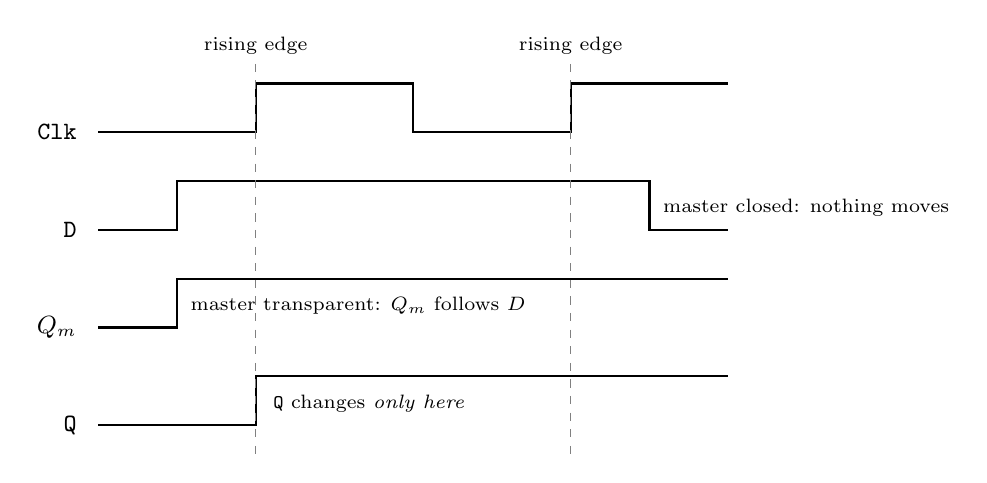
\begin{tikzpicture}[x=1.0cm, y=0.62cm]
  \node[left] at (-0.15, 0) {\small\code{Clk}};
  \draw[thick] (0,0) -- (2,0) -- (2,1) -- (4,1) -- (4,0) -- (6,0) -- (6,1) -- (8,1);
  \node[left] at (-0.15,-2) {\small\code{D}};
  \draw[thick] (0,-2) -- (1,-2) -- (1,-1) -- (7,-1) -- (7,-2) -- (8,-2);
  \node[left] at (-0.15,-4) {\small$Q_m$};
  \draw[thick] (0,-4) -- (1,-4) -- (1,-3) -- (8,-3);
  \node[left] at (-0.15,-6) {\small\code{Q}};
  \draw[thick] (0,-6) -- (2,-6) -- (2,-5) -- (8,-5);
  \foreach \x in {2,6} \draw[dashed,gray] (\x,1.4) -- (\x,-6.6);
  \node[above] at (2,1.4) {\scriptsize rising edge};
  \node[above] at (6,1.4) {\scriptsize rising edge};
  \node[right,font=\scriptsize] at (1.05,-3.55) {master transparent: $Q_m$ follows $D$};
  \node[right,font=\scriptsize] at (2.1,-5.55) {\code{Q} changes \emph{only here}};
  \node[right,font=\scriptsize] at (7.05,-1.55) {master closed: nothing moves};
\end{tikzpicture}
\end{center}

\subsection*{1.2 Equations --- nothing new was invented}

\begin{align*}
\text{master} \quad & Q_m^{+} = \overline{Clk}\cdot D + Clk\cdot Q_m \\
\text{slave}  \quad & Q^{+}   = Clk\cdot Q_m + \overline{Clk}\cdot Q
\end{align*}

Both are Lab 1's latch, $Q^{+} = En\cdot D + \overline{En}\cdot Q$, with
$\overline{Clk}$ and $Clk$ connected to $En$. \textbf{``Edge-triggered'' is not a
primitive. It is a consequence.}

\subsection*{1.3 The code, and the one line that does the work}

\begin{lstlisting}
ClkN <= not Clk;                       -- the opposite enable: the whole trick

MASTER : entity work.trans_latch
    port map ( D => D,  En => ClkN, Q => Qm );
SLAVE  : entity work.trans_latch
    port map ( D => Qm, En => Clk,  Q => Q  );
\end{lstlisting}

This is \textbf{structural VHDL in the strict sense}: components joined by
signals. The two instances are the same component; they differ only in what is
connected to \code{En} and \code{D}, which is exactly why named association
matters here.

\code{Qm} is the wire between them. \textbf{Add it to the wave window} --- it is
the only place the mechanism is visible.

\subsection*{1.4 The testbench, and its key vector}

\begin{center}
\small
\begin{tabular}{>{\raggedright\arraybackslash}p{6.0cm}>{\raggedright\arraybackslash}p{8.2cm}}
\toprule
stimulus & what the check proves \\
\midrule
settle two periods with \code{D} low & the output starts from a known value \\
raise \code{D} between edges, check 1~ns later & \code{Q} does \textbf{not} follow \code{D} between edges \\
wait for the rising edge & \code{Q} captured \code{D} \emph{at} the edge \\
\textbf{toggle \code{D} three times inside one period} & \textbf{the key vector:} \code{Q} ignores all of it \\
wait for the next rising edge & \code{Q} takes the \textbf{last} value before the edge \\
\bottomrule
\end{tabular}
\end{center}

\begin{lstlisting}
wait until falling_edge(Clk);
D <= '0'; wait for 2 ns;
D <= '1'; wait for 2 ns;
D <= '0'; wait for 2 ns;
check('1', "Q ignores all toggling between edges");
\end{lstlisting}

\textbf{Two timing habits to point at explicitly:}

\begin{itemize}[leftmargin=1.6em,itemsep=1pt]
\item Stimulus changes just after a \textbf{falling} edge --- as far from the next
rising edge as possible. Changing \code{D} \emph{on} a rising edge is a setup-time
violation, and the result is meaningless in simulation and in hardware.
\item Checks happen \textbf{1~ns after} the rising edge, never at it. At the edge
itself the new value has not propagated, and you would read the old one.
\end{itemize}

\textbf{The clock generator needs \code{wait for}}, and the \code{running} flag
lets the run finish. A clock process with no \code{wait} loops at time zero
without advancing time: the simulator looks frozen but is actually spinning.

\vspace{4pt}\hr

\section*{Example 2 --- Same behaviour, different structure}

\subsection*{2.1 The two descriptions}

\begin{lstlisting}
-- structural: two latches, an inverter, and a wire called Qm
-- behavioural:
process (Clk)
begin
    if rising_edge(Clk) then
        Q <= D;
    end if;
end process;
\end{lstlisting}

\textbf{Note the sensitivity list: \code{(Clk)} only, and that is correct here.} A
clocked process reacts to the clock, not to the data --- \code{D} is read only at
the edge. This is the opposite of Lab 1's rule, and it is the rule your
\code{RegN} needs (with \code{Rst} added, because the reset is asynchronous).

\subsection*{2.2 The testbench asserts they agree}

Both flip-flops see identical stimulus, and every check compares them to each
other rather than to a constant:

\begin{lstlisting}
if Q_struct /= Q_behav then
    report "FAIL: ..." severity error;
\end{lstlisting}

\textbf{If the two descriptions really are the same hardware, no check can ever
fail.} That is the claim being tested, and it is a pattern worth reusing: when you
have two implementations, the cheapest strong test is to assert they agree on
every vector.

\subsection*{2.3 Same waveform, different hardware --- measured}

\begin{center}
\begin{tabular}{lcc}
\toprule
& \code{ms\_flipflop} (structural) & behavioural \code{dff} \\
\midrule
Total registers & \textbf{0} & \textbf{1} \\
Inferred latches & \textbf{2} & 0 \\
Netlist primitives & 2 LUTs & 1 flip-flop (\code{arriav\_ff}) \\
RTL Viewer & two latch symbols $+$ inverter & one flip-flop symbol \\
Waveform & \multicolumn{2}{c}{\textbf{indistinguishable}} \\
\bottomrule
\end{tabular}
\end{center}

\textbf{Read that table aloud in the report.} You built a flip-flop and the tool
reported two latches, because that is literally what you asked for. The
behavioural version names the \emph{idiom} \code{rising\_edge(Clk)}, which the
synthesiser maps onto the FPGA's dedicated flip-flop --- smaller and faster than
two latches built out of LUTs.

\textbf{Which would you ship?} The behavioural one, everywhere. The structural one
exists so you know what the primitive is made of. \emph{You describe intent; the
tool chooses an implementation.}

\subsection*{2.4 A naming trap, measured}

The example entity is called \code{dff}, which collides with a device primitive of
the same name. It simulates fine, but set it as the top level and Quartus says:

\begin{lstlisting}[language={},numbers=none]
Error (12007): Top-level design entity "dff" is undefined
\end{lstlisting}

Renaming it (for example to \code{dff\_beh}) compiles and reports 1 register. The
same applies to \code{and2}, \code{or3} and other primitive names. \textbf{An
entity that plainly exists, reported as undefined, is usually a name that already
belongs to the tool.}

\vspace{4pt}\hr

\section*{Example 3 --- One entity, every width}

\subsection*{3.1 The generic}

\begin{lstlisting}
entity reg_n is
    generic ( N : positive := 8 );          -- compile-time parameter
    port (
        D   : in  std_logic_vector(N - 1 downto 0);
        Clk : in  std_logic;
        Ld  : in  std_logic;
        Rst : in  std_logic;
        Q   : out std_logic_vector(N - 1 downto 0)
    );
end entity reg_n;
\end{lstlisting}

A \code{generic} is a \textbf{compile-time parameter}. One entity replaces
\code{reg4}, \code{reg5}, \code{reg8} and \code{reg32}. The CPU needs 5-bit
registers for register numbers and 32-bit registers for data, and both come from
this file without editing it.

\begin{lstlisting}
R5  : entity work.reg_n generic map (N => 5)
      port map (D => D5, Clk => Clk, Ld => Ld, Rst => Rst, Q => Q5);
\end{lstlisting}

\textbf{\code{generic map} comes first, and there is no semicolon between it and
\code{port map}} --- they are one statement. Forget the \code{generic map} and you
silently get the default width; the error then appears at the signal you
connected, not at the instance that is wrong.

\subsection*{3.2 The table, and why it is Lab 1's table}

\begin{center}
\begin{tabular}{c|ccc|c|l}
\toprule
\# & \code{Rst} & \code{Ld} & \code{Clk} & $Q^{+}$ & note \\
\midrule
0 & 1 & -- & -- & \textbf{0} & asynchronous reset \\
1 & 0 & -- & not $\uparrow$ & $\mathbf{Q}$ & hold between edges \\
2 & 0 & 0 & $\uparrow$ & $\mathbf{Q}$ & edge, but not loading \\
3 & 0 & 1 & $\uparrow$ & $\mathbf{D}$ & load \\
\bottomrule
\end{tabular}
\end{center}

\[
Q_i^{+} = \overline{\code{Rst}}\cdot\left( \code{Ld}\cdot D_i + \overline{\code{Ld}}\cdot Q_i \right)
\qquad\text{compare Lab 1:}\qquad
Q^{+} = \overline{\code{Clr}}\cdot\left( \code{En}\cdot D + \overline{\code{En}}\cdot Q \right)
\]

\textbf{The same equation.} \code{En} became \code{Ld}, \code{Clr} became
\code{Rst}, and the enable is now sampled at an edge instead of continuously.

\subsection*{3.3 The three structural details}

\textbf{(a) \code{Rst} is tested outside the edge test}, which is what makes it
asynchronous. Moving it inside \code{rising\_edge} gives a synchronous reset ---
a different circuit, and it contradicts row 0.

\textbf{(b) \code{Ld} goes in a nested \code{if}}, not as
\code{elsif rising\_edge(Clk) and Ld = '1'}. Both simulate identically, but the
nested form keeps the edge test as the only condition on the \code{elsif}, which
is the pattern synthesisers recognise. The other form can produce gated-clock
logic.

\textbf{(c) Row 2 is the missing \code{else}} --- the same VHDL rule as Lab 1
(``no assignment means hold''), now inside a clocked process. \textbf{Identical
rule, different hardware:} last week it produced a latch, this week a register
with a load enable.

\subsection*{3.4 Sensitivity list --- the rule that changed}

\begin{center}
\begin{tabular}{lll}
\toprule
& Lab 1 (latch) & Lab 2 (register) \\
\midrule
rule & every signal the process \emph{reads} & the clock $+$ asynchronous controls only \\
list & \code{(Clr, En, D)} & \code{(Clk, Rst)} \\
\bottomrule
\end{tabular}
\end{center}

\code{Ld} and \code{D} are read only at the edge, and the process is already awake
then because \code{Clk} changed.

\vspace{4pt}\hr

\section*{Into the assignment}

\begin{center}
\begin{tabular}{ll}
\toprule
example & becomes \\
\midrule
\code{ms\_flipflop} & \code{MSFlipFlop}: the same build \textbf{plus \code{Clr} to both latches} \\
\code{dff} & the behavioural style you use for every clocked design from now on \\
\code{reg\_n} & \code{RegN}: default 32, instantiated at 5 and at 32 \\
\bottomrule
\end{tabular}
\end{center}

The one thing the examples do \emph{not} show you is the asynchronous clear on the
flip-flop. It must reach \textbf{both} latches: clear the slave alone and the
master pushes the old value back at the very next rising edge, so the clear
appears to undo itself one cycle later.

\vspace{6pt}
\hr
{\small \textbf{Forward.} \code{RegN} is the most reused component in the course:
32 of them make the register file in Lab 6, one becomes the program counter in
Lab 7, and both appear inside the CPU in Lab 12.}

\end{document}
